\documentclass[tikz,border=7pt]{standalone}
\usepackage[scaled=0.95]{helvet}
\renewcommand{\familydefault}{\sfdefault}
\usepackage{tikz}
\definecolor{TEJNavy}{HTML}{1E2B55}
\definecolor{TEJBlue}{HTML}{1769AA}
\begin{document}
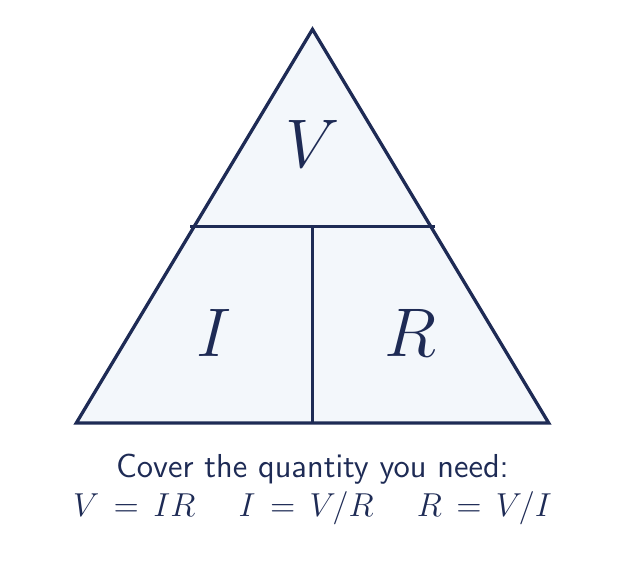
\begin{tikzpicture}[draw=TEJNavy,text=TEJNavy,line width=1.2pt]
  \coordinate (top) at (0,3.5);
  \coordinate (left) at (-3.0,-1.5);
  \coordinate (right) at (3.0,-1.5);
  \draw[fill=TEJBlue!5] (top) -- (left) -- (right) -- cycle;
  \draw (-1.55,1.0) -- (1.55,1.0);
  \draw (0,1.0) -- (0,-1.5);

  \node[font=\bfseries\fontsize{30}{32}\selectfont] at (0,2.05) {$V$};
  \node[font=\bfseries\fontsize{30}{32}\selectfont] at (-1.25,-0.35) {$I$};
  \node[font=\bfseries\fontsize{30}{32}\selectfont] at (1.25,-0.35) {$R$};

  \node[font=\large,align=center,text width=7.0cm] at (0,-2.35)
    {Cover the quantity you need: $V=IR$ \quad $I=V/R$ \quad $R=V/I$};
\end{tikzpicture}
\end{document}
